\afterpage{
    \clearpage

    \begin{figure*}
        \centering
        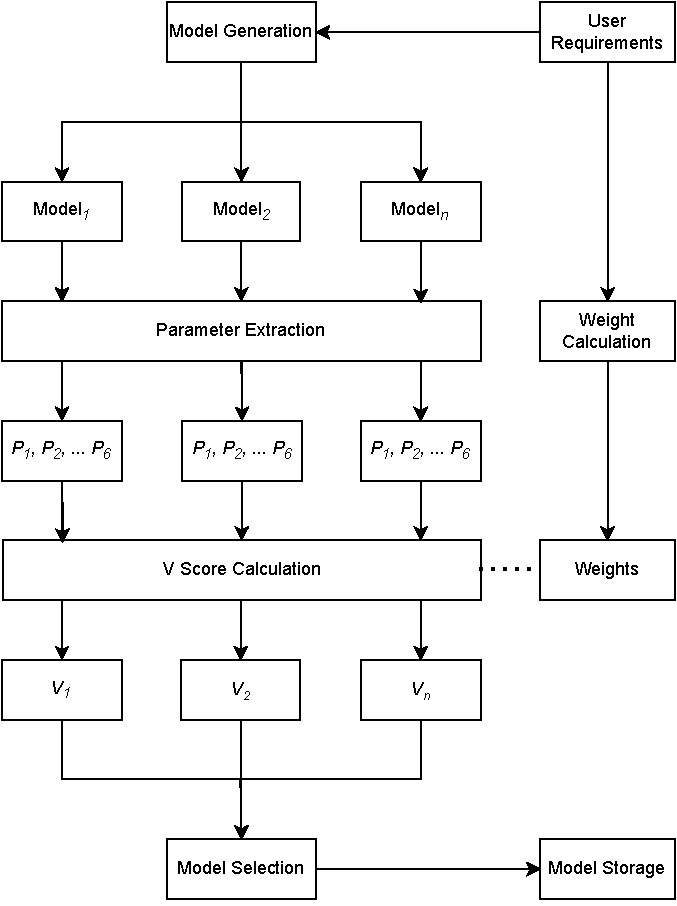
\includegraphics[width=1.4\columnwidth]{media/ch_dataset_and_methods/math_model_relaxed.pdf}
        \caption{Model Selection Approach}
        \label{fig:model_selection_approach}
    \end{figure*}

    % Best model Performance chart
    \begin{figure*}[ht]
        \centering
        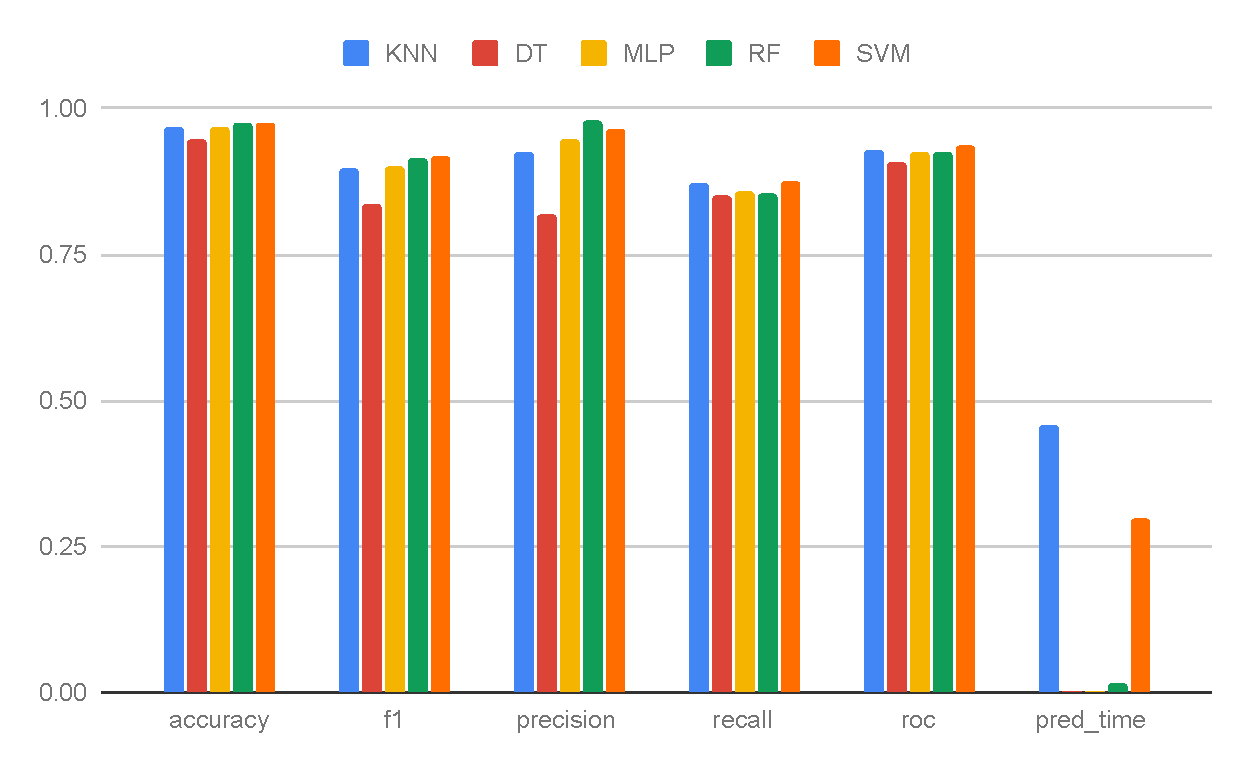
\includegraphics[width=1.9\columnwidth]{media/ch_result_and_testing/perf_ds_1.pdf}
        \caption{Performance Results Dataset 1} \label{fig:perfromance_results_dataset_1}
    \end{figure*}

    \begin{figure*}[ht]
        \centering
        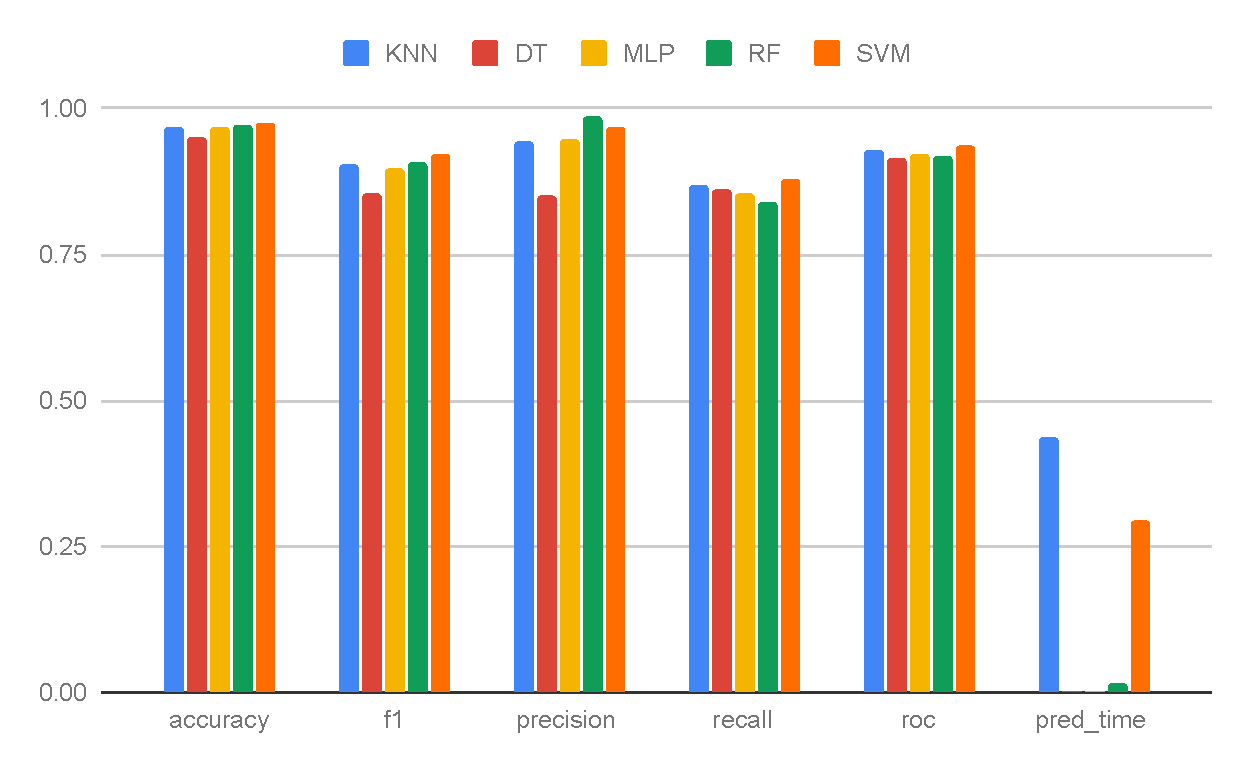
\includegraphics[width=1.9\columnwidth]{media/ch_result_and_testing/perf_ds_2.pdf}
        \caption{Performance Results Dataset 2} \label{fig:perfromance_results_dataset_2}
    \end{figure*}

    \begin{figure*}[ht]
        \centering
        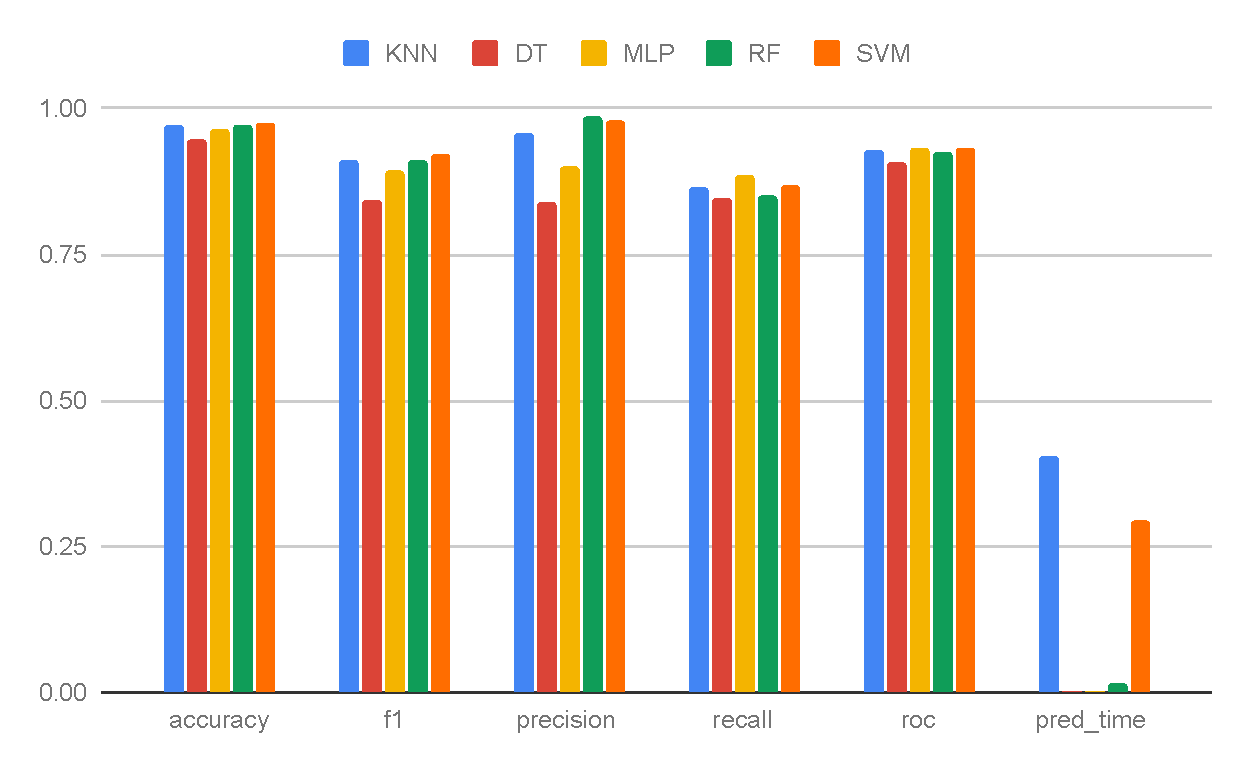
\includegraphics[width=1.9\columnwidth]{media/ch_result_and_testing/perf_ds_3.pdf}
        \caption{Performance Results Dataset 3} \label{fig:perfromance_results_dataset_3}
    \end{figure*}

    \begin{figure*}[ht]
        \centering
        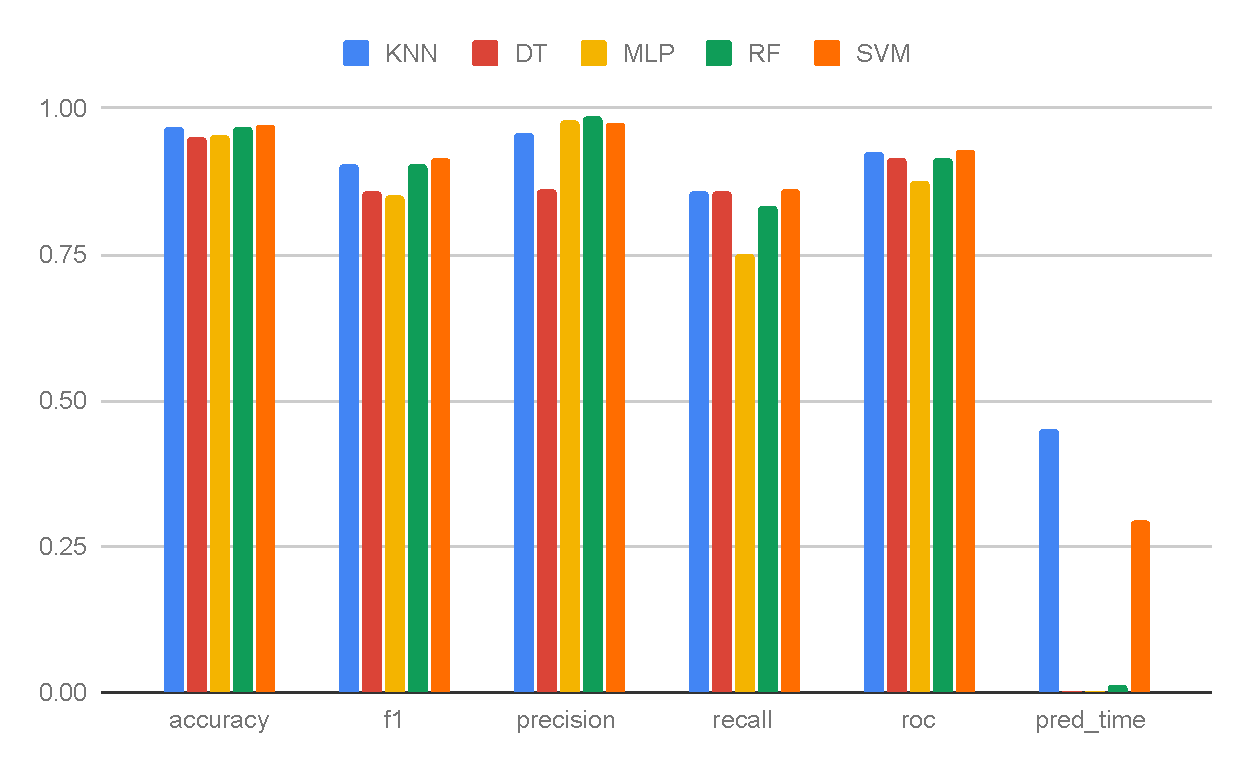
\includegraphics[width=1.9\columnwidth]{media/ch_result_and_testing/perf_ds_4.pdf}
        \caption{Performance Results Dataset 4} \label{fig:perfromance_results_dataset_4}
    \end{figure*}

    \begin{figure*}[ht]
        \centering
        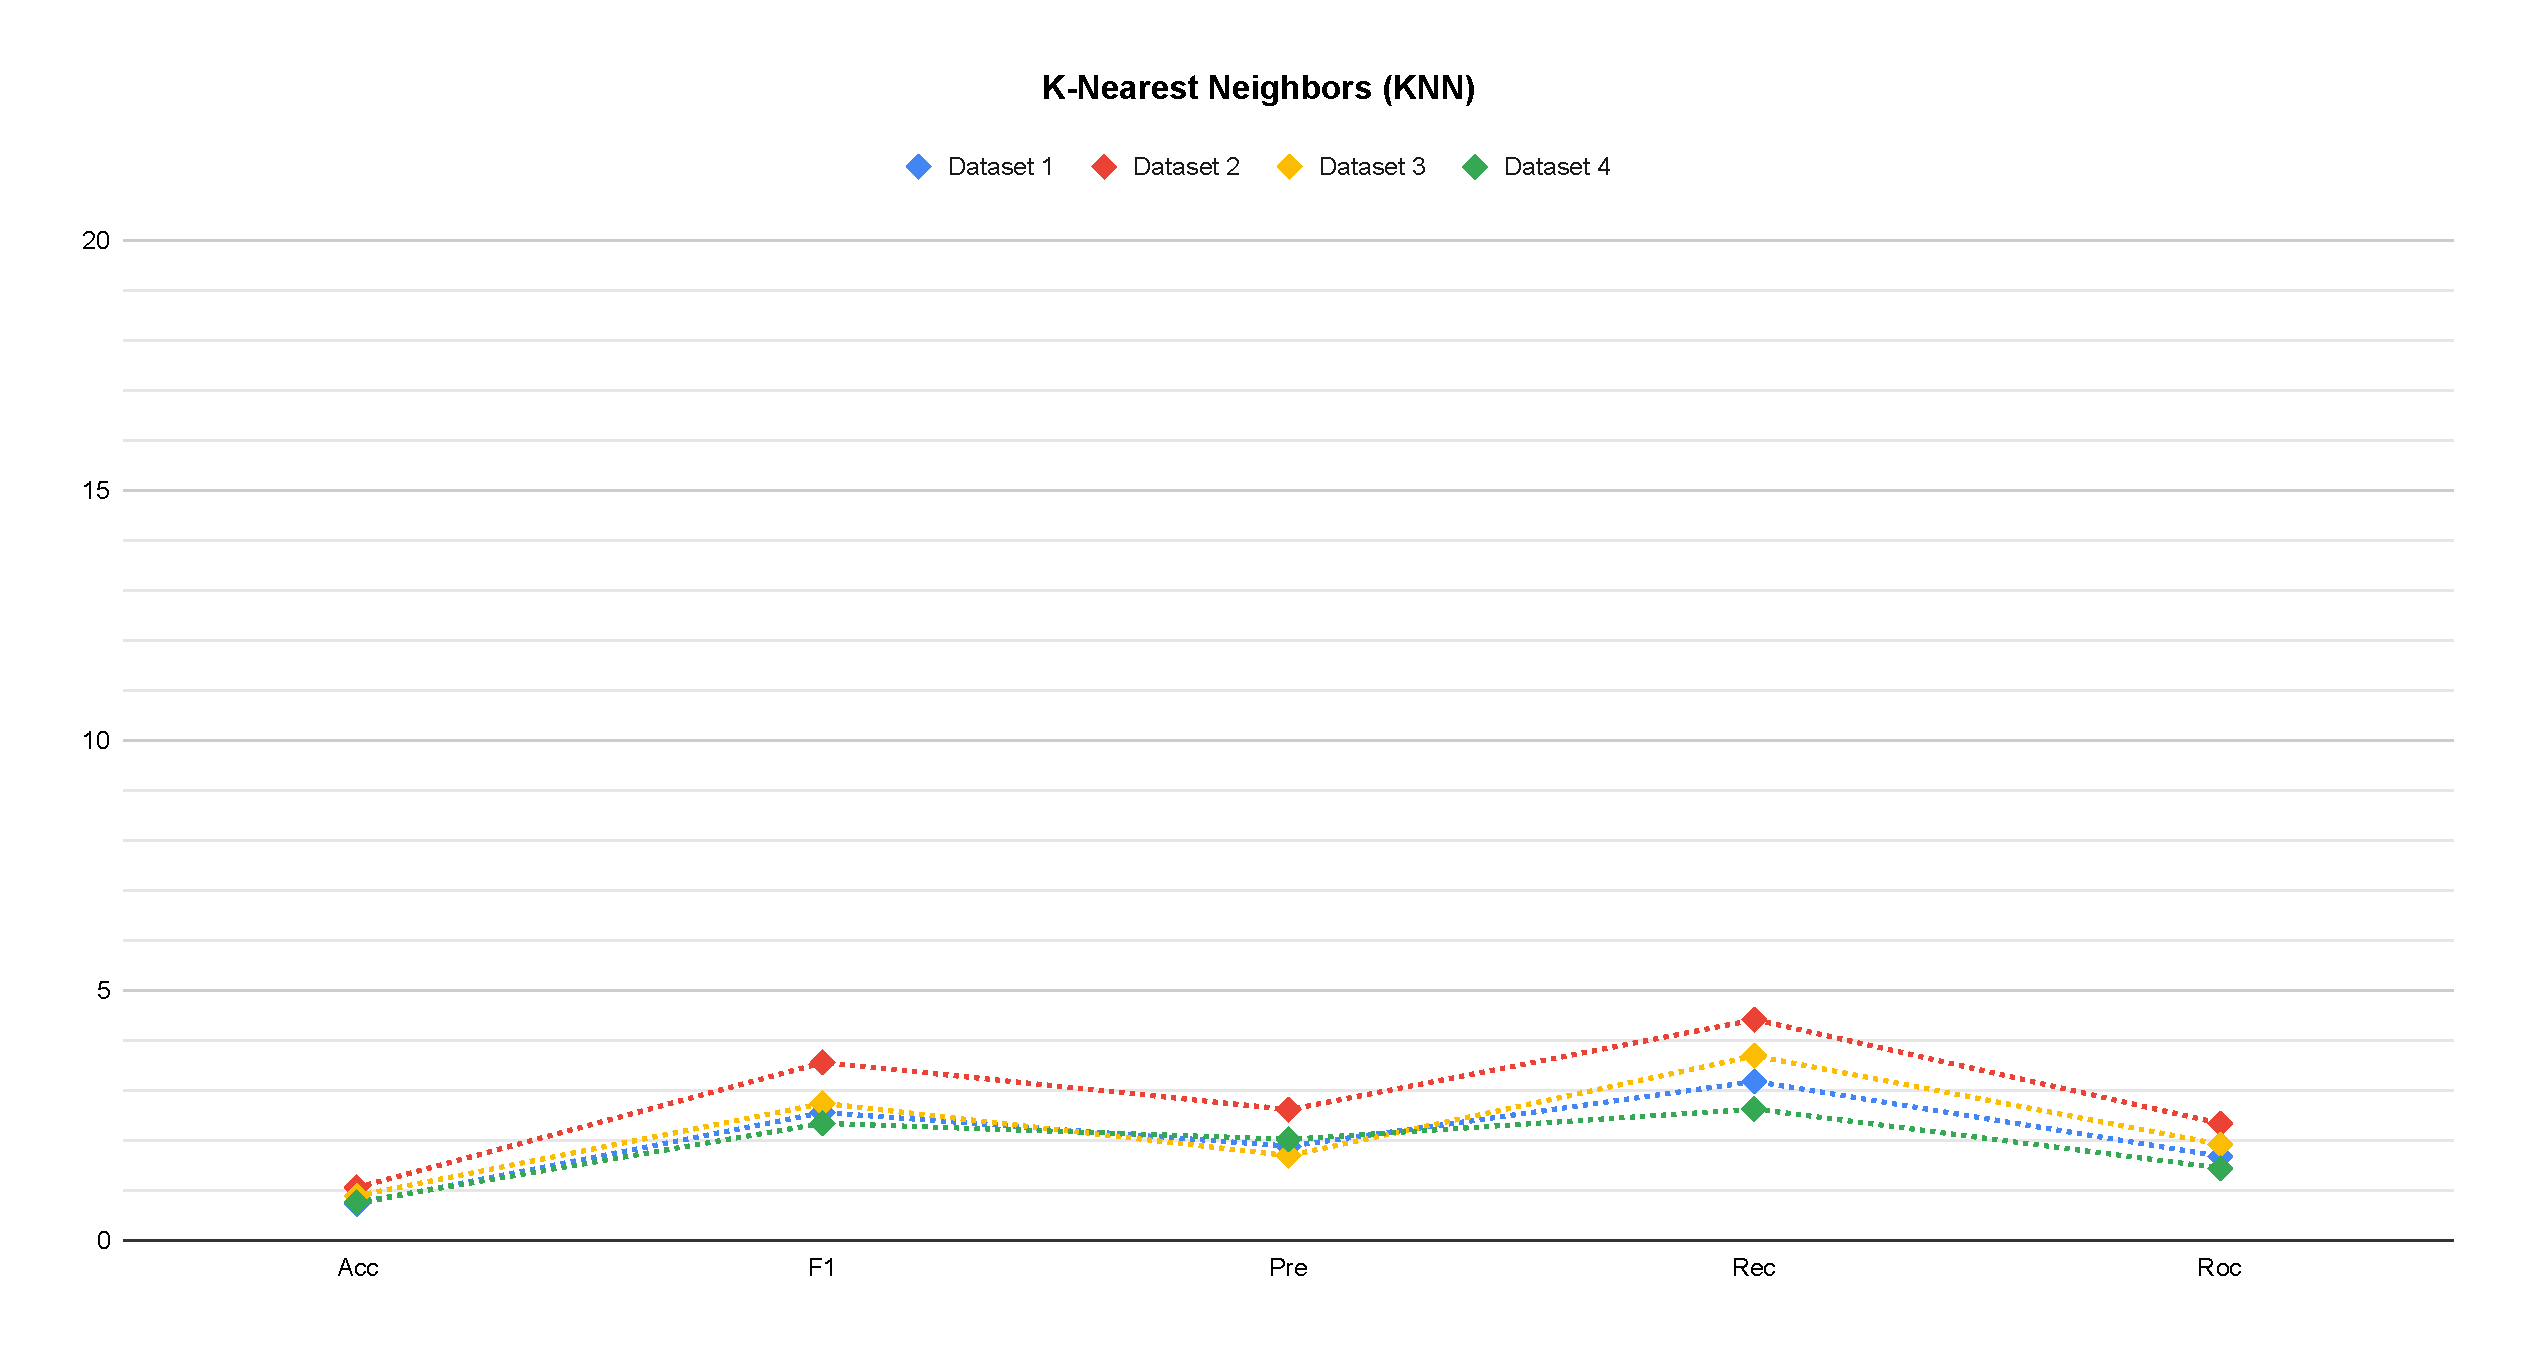
\includegraphics[width=1.9\columnwidth]{media/ch_result_and_testing/delta_KNN.pdf}
        \caption{Average Error for K-Nearest Neighbors (KNN) model} \label{fig:perfromance_delta_knn}
    \end{figure*}

    \begin{figure*}[ht]
        \centering
        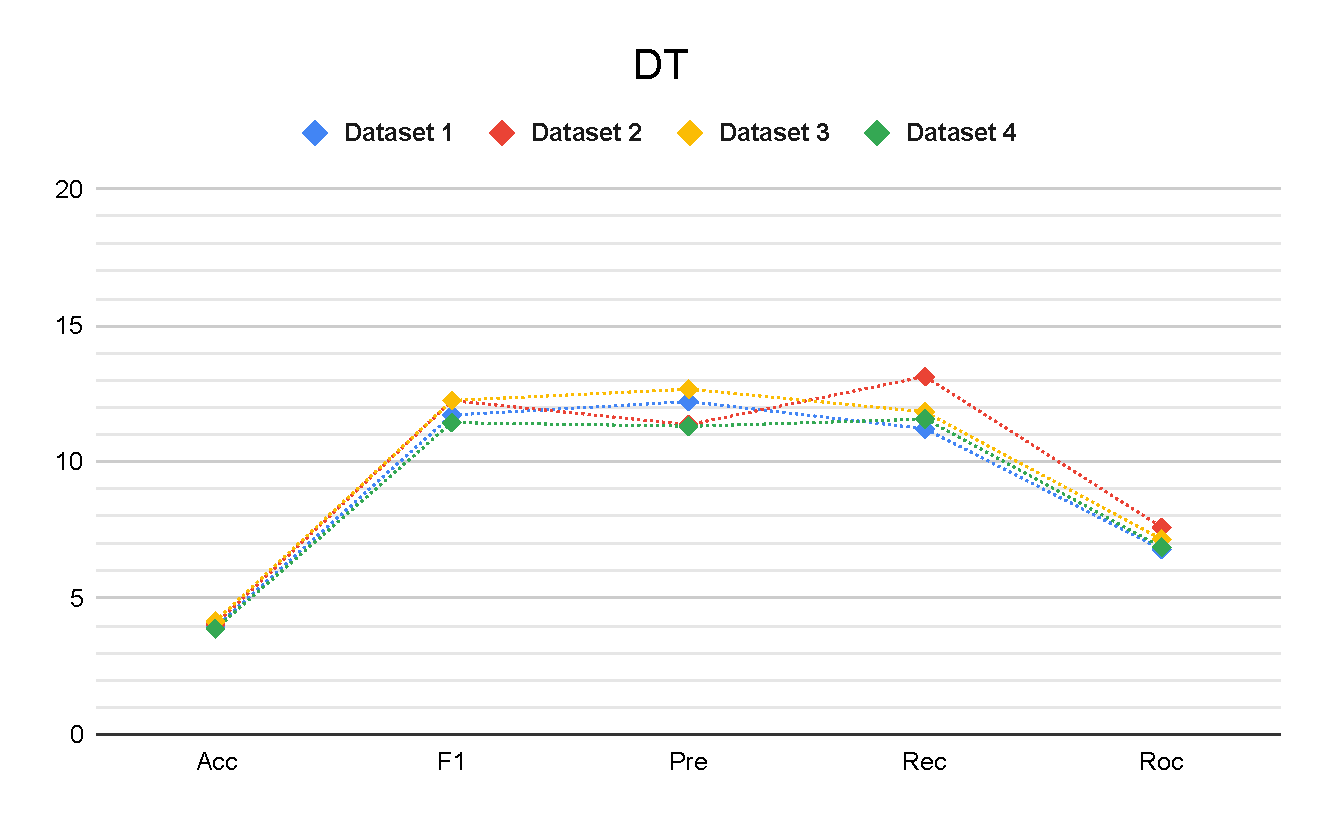
\includegraphics[width=1.9\columnwidth]{media/ch_result_and_testing/delta_DT.pdf}
        \caption{Average Error for Decision Tree (DT) model} \label{fig:perfromance_delta_dt}
    \end{figure*}

    \begin{figure*}[ht]
        \centering
        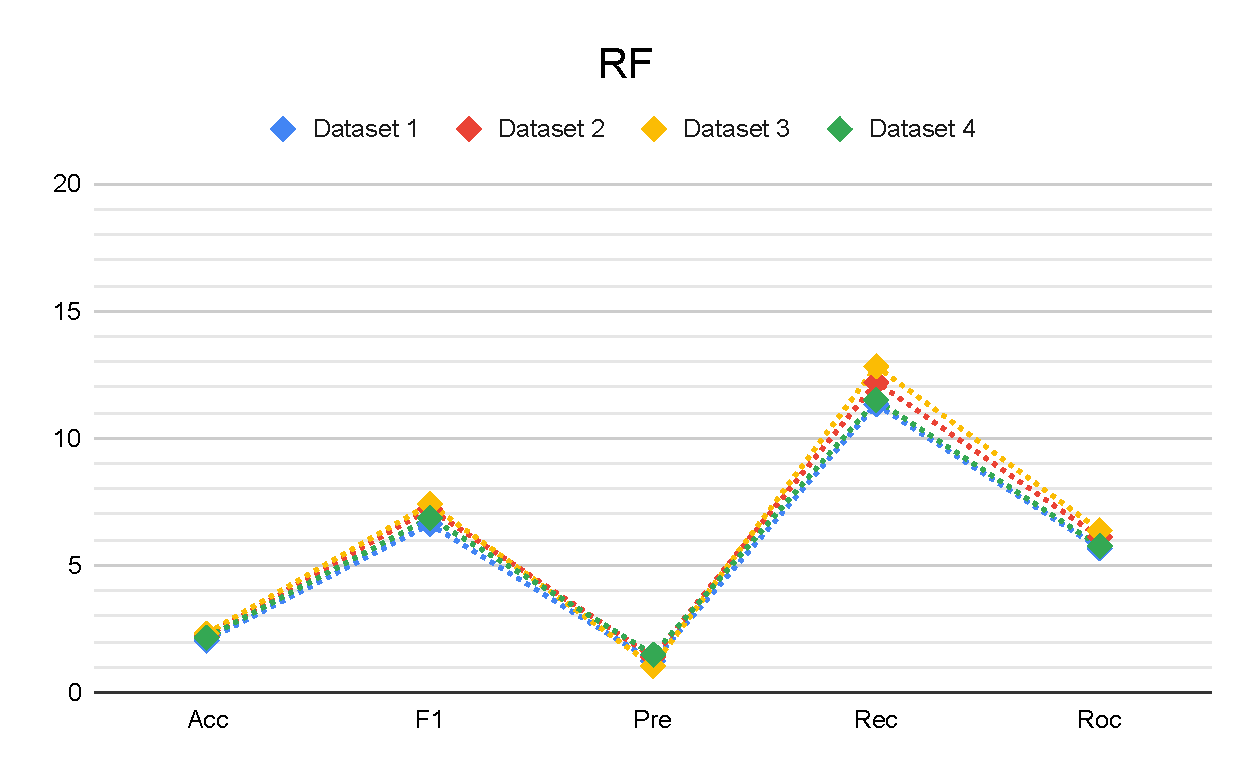
\includegraphics[width=1.9\columnwidth]{media/ch_result_and_testing/delta_RF.pdf}
        \caption{Average Error for Random Forest (RF) model} \label{fig:perfromance_delta_rf}
    \end{figure*}

    \begin{figure*}[ht]
        \centering
        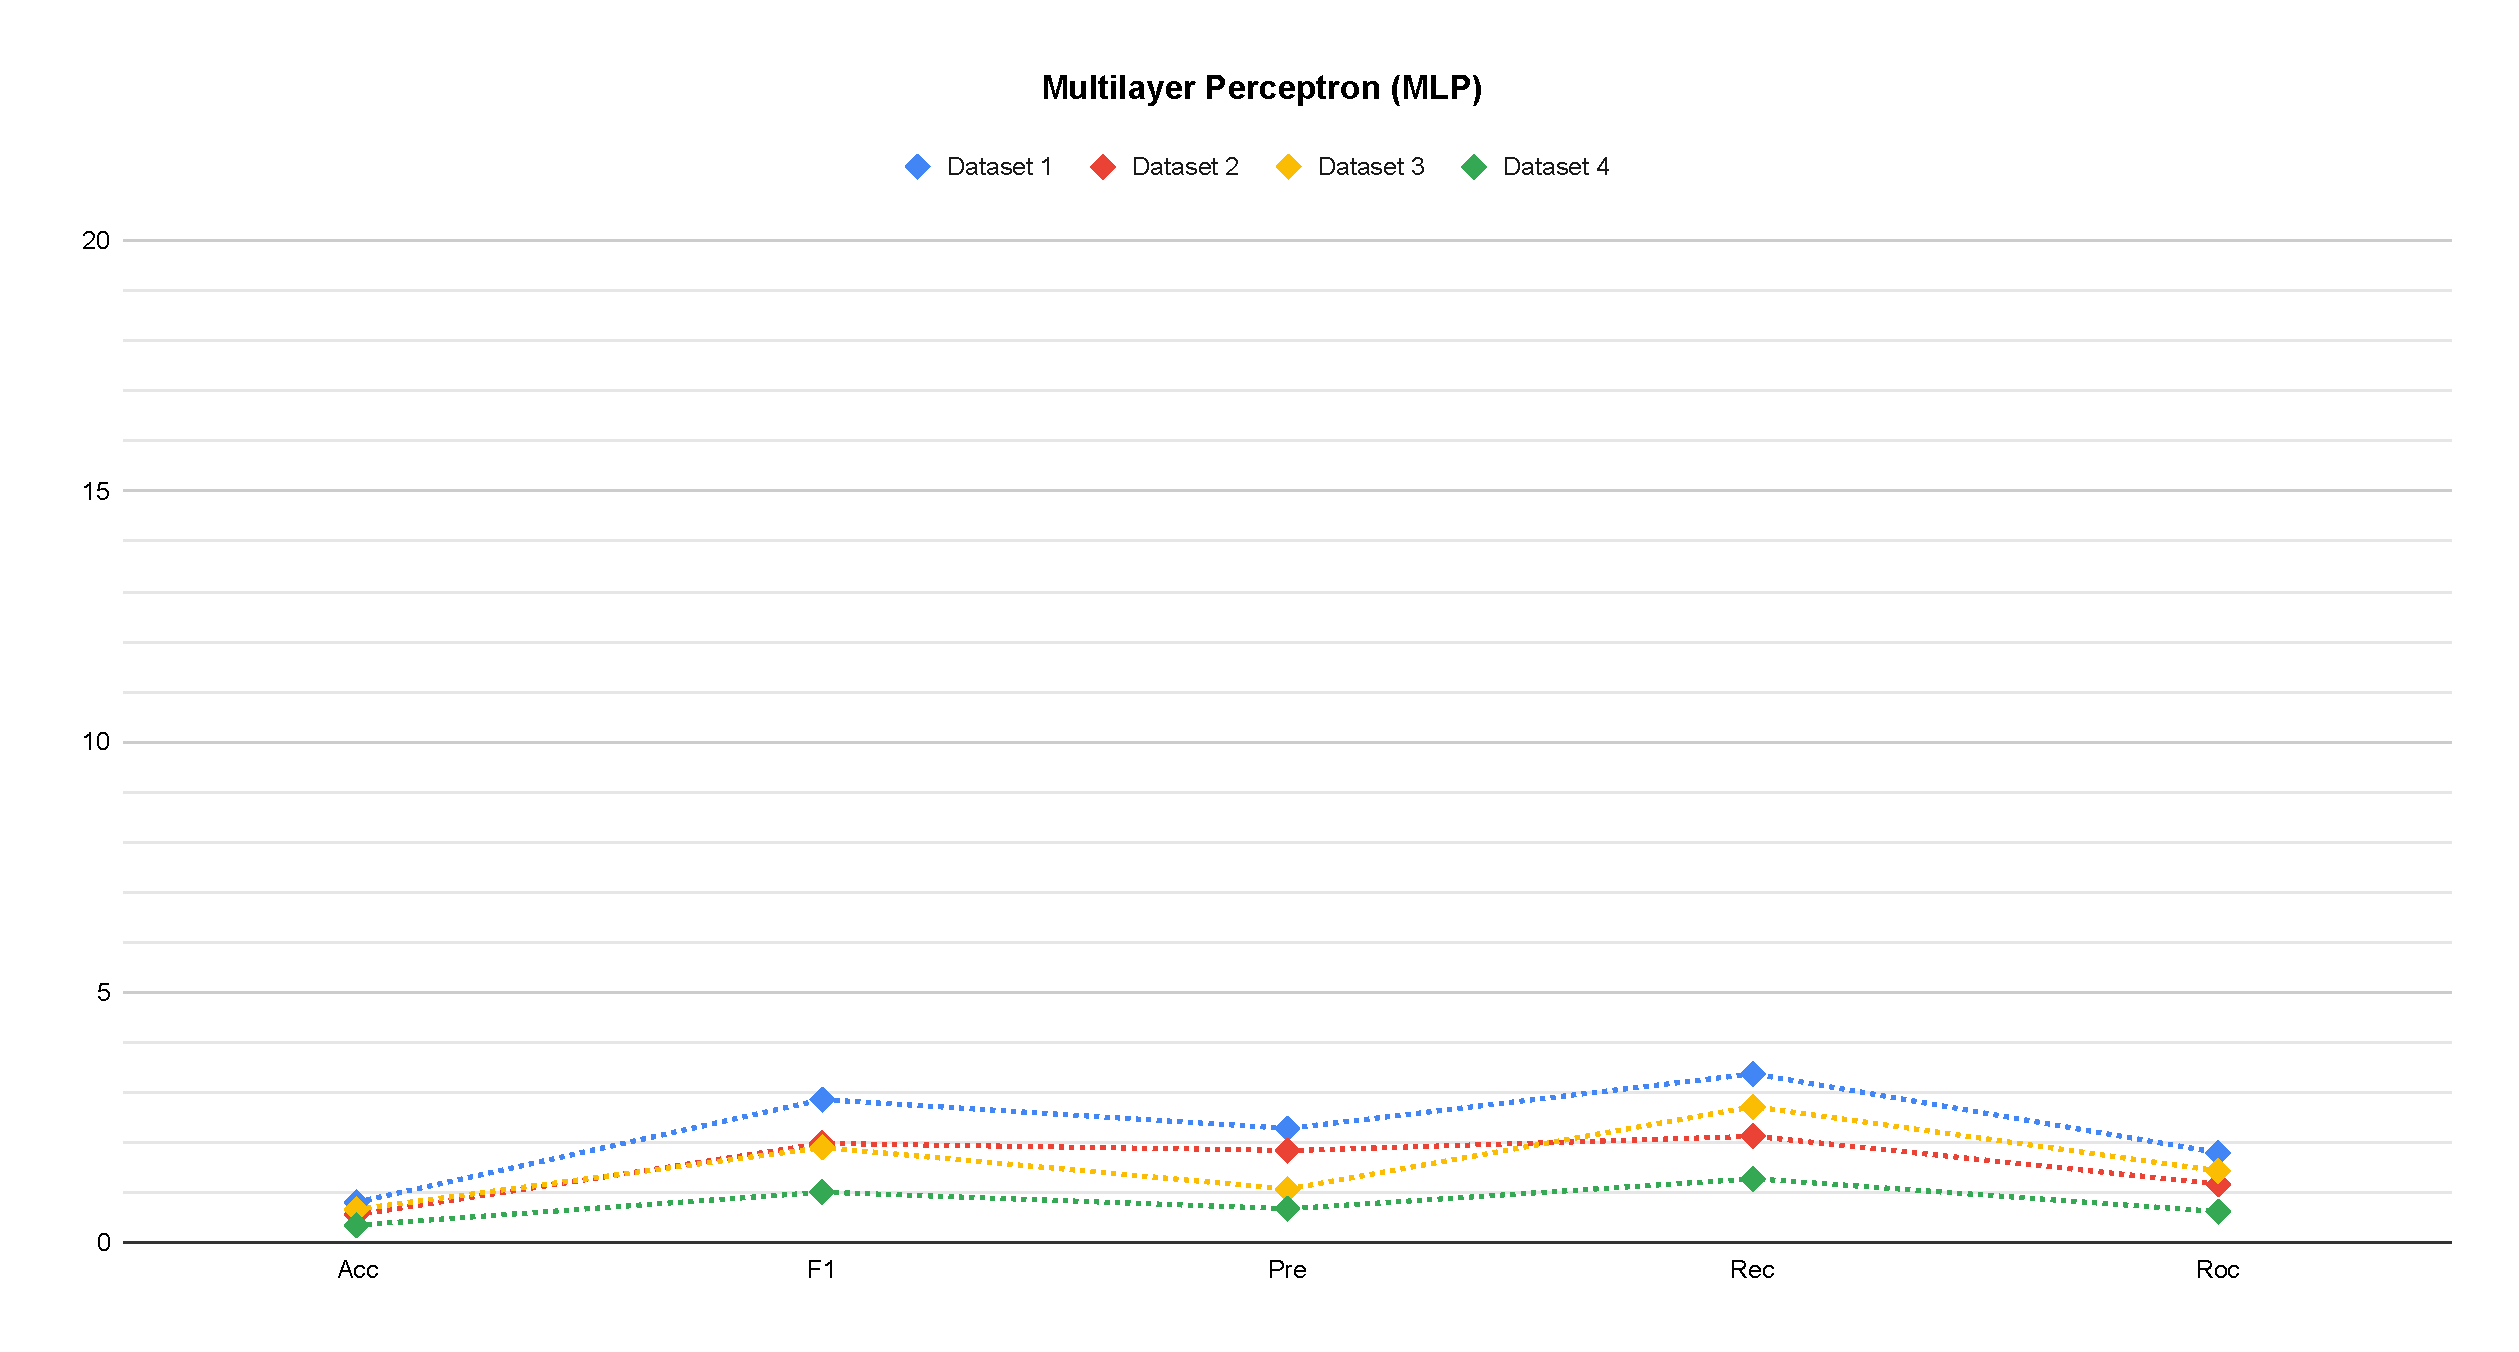
\includegraphics[width=1.9\columnwidth]{media/ch_result_and_testing/delta_MLP.pdf}
        \caption{Average Error for Multilayer Perceptron (MLP) model} \label{fig:perfromance_delta_mlp}
    \end{figure*}

    \begin{figure*}[ht]
        \centering
        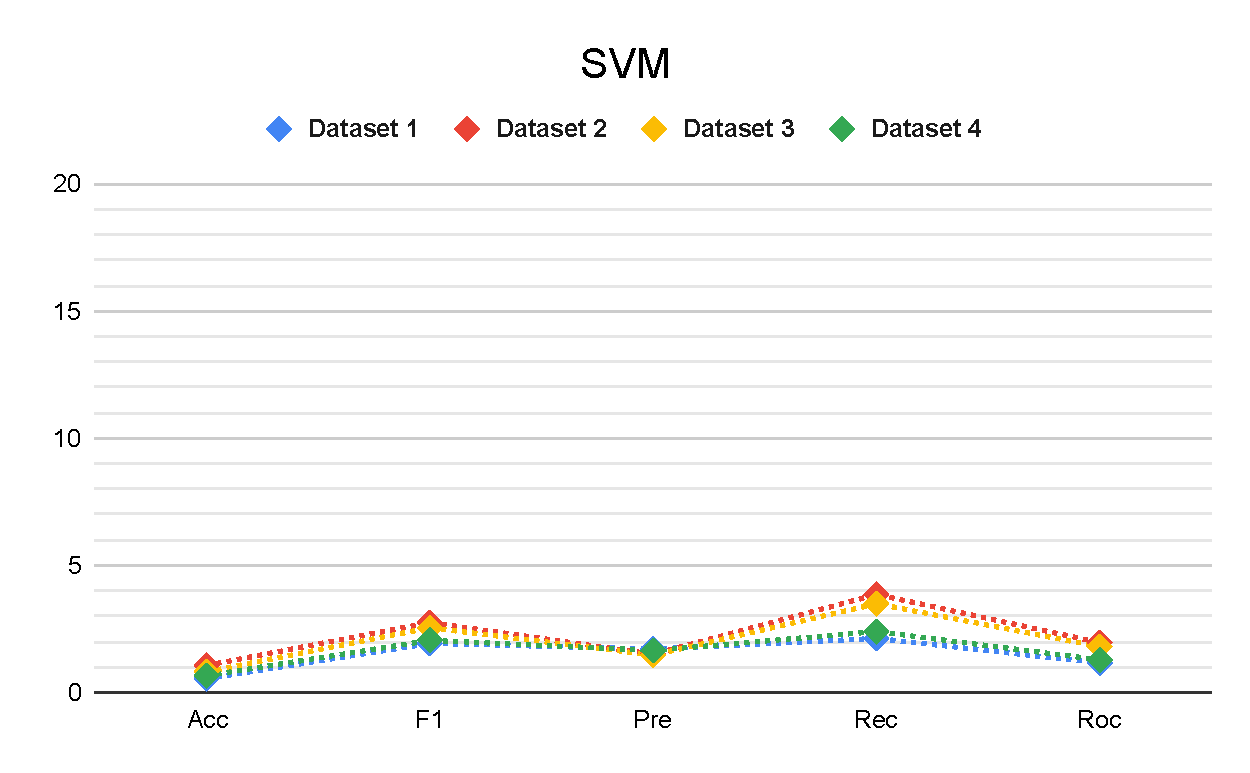
\includegraphics[width=1.9\columnwidth]{media/ch_result_and_testing/delta_SVM.pdf}
        \caption{Average Error for Support Vector Machine (SVM) model} \label{fig:perfromance_delta_svm}
    \end{figure*}

    \clearpage
    \begin{table}[H]
        {\responsemod
            \caption{Vscores of Models}\label{tab:vscores_models}
            \begin{tabular*}{\tblwidth}{@{}FKKKK@{}}
                \toprule
                \bfrow Models & Dataset 1 & Dataset 2 & Dataset 3 & Dataset 4 \\
                \midrule
                KNN & 2.747 & 2.758 & 2.774 & 2.760 \\
                DT & 2.643 & 2.684 & 2.658 & 2.687 \\
                MLP & 2.782 & 2.771 & 2.766 & 2.674 \\
                RF & \textbf{2.807} & 2.795 & 2.803 & 2.786 \\
                SVM & 2.482 & \textbf{2.808} & \textbf{2.803} & \textbf{2.790} \\
                \bottomrule
            \end{tabular*}
        }
    \end{table}

    % Best model Performance tabular
    \begin{table}[hbt]
        \caption{Performance of models trained on dataset 1} \label{tab:performance_of_models_trained_on_dataset_1}
        \begin{tabular*}{\tblwidth}{@{}FKKKHK@{}}
            \toprule
            \bfrow Metric & KNN$_1$ & DT$_1$ & MLP$_1$ & RF$_1$ & SVM$_1$ \\
            \midrule
            Accuracy & 96.72 & 94.46 & 96.89 & 97.33 & 97.40 \\
            F1 & 89.71 & 83.43 & 90.05 & 91.30 & 91.69 \\
            Precision & 92.53 & 81.86 &94.71 &  97.95 & 96.43 \\
            Recall & 87.06 & 85.06 & 85.84 & 85.50 & 87.40 \\
            ROC & 92.84 & 90.68 & 92.45 & 92.57 & 93.38 \\
            Time(s) & 0.457 & 0.001 & 0.002 & 0.015 & 0.297 \\
            \bluerow V$_{score}$ & 2.747 & 2.643 & 2.782 & 2.807 & 2.482 \\
            \bottomrule
        \end{tabular*}
    \end{table}

    \begin{table}[hbt]
        \caption{Performance of models trained on dataset 2} \label{tab:performance_of_models_trained_on_dataset_2}
        \begin{tabular*}{\tblwidth}{@{}FKKKKH@{}}
            \toprule
            \bfrow Metric & KNN$_2$ & DT$_2$ & MLP$_2$ & RF$_2$ & SVM$_2$ \\
            \midrule
            Accuracy & 96.83 & 95.04 & 96.69 & 97.09 & 97.46 \\
            F1 & 90.28 & 85.50 & 89.73 & 90.75 & 92.15 \\
            Precision & 94.25 & 84.90 & 94.73 & 98.60 & 96.79 \\
            Recall & 86.63 & 86.09 & 85.23 & 84.05 & 87.93 \\
            ROC & 92.77 & 91.48 & 92.13 & 91.90 & 93.66 \\
            Time(s) & 0.435 & 0.001 & 0.003 & 0.014 & 0.295 \\
            \bluerow V$_{score}$ & 2.758 & 2.684 & 2.772 & 2.795 & 2.808 \\
            \bottomrule
        \end{tabular*}
    \end{table}

    \begin{table}[hbt]
        \caption{Performance of models trained on dataset 3} \label{tab:performance_of_models_trained_on_dataset_3}
        \begin{tabular*}{\tblwidth}{@{}FKKKKH@{}}
            \toprule
            \bfrow Metric & KNN$_3$ & DT$_3$ & MLP$_3$ & RF$_3$ & SVM$_3$ \\
            \midrule
            Accuracy & 97.07 & 94.64 & 96.41 & 97.22 & 97.44 \\
            F1 & 90.93 & 84.30 & 89.34 & 91.21 & 92.00 \\
            Precision & 95.82 & 83.81 & 90.13 & 98.37 & 97.81 \\
            Recall & 86.53 & 84.80 & 88.57 & 85.02 & 86.85 \\
            ROC & 92.87 & 90.73 & 93.29 & 92.36 & 93.22 \\
            Time(s) & 0.404 & 0.001 & 0.002 & 0.017 & 0.293 \\
            \bluerow V$_{score}$ & 2.774 & 2.658 & 2.766 & 2.803 & 2.803 \\
            \bottomrule
        \end{tabular*}
    \end{table}

    \begin{table}[hbt]
        \caption{Performance of models trained on dataset 4} \label{tab:performance_of_models_trained_on_dataset_4}
        \begin{tabular*}{\tblwidth}{@{}FKKKKH@{}}
            \toprule
            \bfrow Metric & KNN$_4$ & DT$_4$ & MLP$_4$ & RF$_4$ & SVM$_4$ \\
            \midrule
            Accuracy & 96.84 & 94.99 & 95.34 & 96.88 & 97.15 \\
            F1 & 90.52 & 85.73 & 85.01 & 90.37 & 91.39 \\
            Precision & 95.71 & 85.91 & 97.83 & 98.65 & 97.41 \\
            Recall & 85.86 & 85.55 & 75.15 & 83.37 & 86.07 \\
            ROC & 92.52 & 91.28 & 87.40 & 91.56 & 92.79 \\
            Time(s) & 0.452 & 0.001 & 0.002 & 0.014 & 0.294 \\
            \bluerow V$_{score}$ & 2.760 & 2.687 & 2.674 & 2.786 & 2.790 \\
            \bottomrule
        \end{tabular*}
    \end{table}

    \begin{sidewaystable}
        {\color{blue}
            \caption{Performance of K Nearest Neighbors Models}\label{tab:performance_k_nearest_neighbors_multi}
            \begin{adjustbox}{center}
                \begin{tabular*}{0.9\textwidth}{@{}F|KKKK|KKKK|KKKK|KKKK@{}}
                    \toprule
                    \bfrow\multirow{2}{*}{Metric} & \multicolumn{4}{K}{Dataset 1} & \multicolumn{4}{K}{Dataset 2} & \multicolumn{4}{K}{Dataset 3} & \multicolumn{4}{K}{Dataset 4} \\
                    \bfrow & KNN$_1$ & KNN$_2$ & KNN$_3$ & KNN$_4$ & KNN$_1$ & KNN$_2$ & KNN$_3$ & KNN$_4$ & KNN$_1$ & KNN$_2$ & KNN$_3$ & KNN$_4$ & KNN$_1$ & KNN$_2$ & KNN$_3$ & KNN$_4$ \\
                    \midrule
                    Accuracy & 0.97 & 0.96 & 0.96 & 0.96 & 0.97 & 0.97 & 0.96 & 0.96 & 0.97 & 0.96 & 0.97 & 0.96 & 0.96 & 0.96 & 0.96 & 0.97 \\
                    F1 & 0.93 & 0.90 & 0.90 & 0.90 & 0.91 & 0.93 & 0.90 & 0.90 & 0.90 & 0.90 & 0.93 & 0.90 & 0.90 & 0.89 & 0.90 & 0.92 \\
                    Precision & 0.96 & 0.94 & 0.95 & 0.94 & 0.95 & 0.96 & 0.95 & 0.95 & 0.94 & 0.94 & 0.96 & 0.94 & 0.94 & 0.94 & 0.94 & 0.96 \\
                    Recall & 0.90 & 0.86 & 0.86 & 0.86 & 0.87 & 0.90 & 0.86 & 0.86 & 0.87 & 0.86 & 0.89 & 0.87 & 0.87 & 0.85 & 0.86 & 0.89 \\
                    ROC & 0.94 & 0.92 & 0.92 & 0.92 & 0.93 & 0.94 & 0.92 & 0.92 & 0.93 & 0.92 & 0.94 & 0.93 & 0.93 & 0.92 & 0.92 & 0.94 \\
                    \bottomrule
                \end{tabular*}
            \end{adjustbox}
        }
    \end{sidewaystable}

    \begin{sidewaystable}
        {\color{blue}
            \caption{Performance of Decision Tree Models}\label{tab:performance_decision_tree_multi}
            \begin{adjustbox}{center}
                \begin{tabular*}{0.9\textwidth}{@{}F|KKKK|KKKK|KKKK|KKKK@{}}
                    \toprule
                    \bfrow\multirow{2}{*}{Metric} & \multicolumn{4}{K}{Dataset 1} & \multicolumn{4}{K}{Dataset 2} & \multicolumn{4}{K}{Dataset 3} & \multicolumn{4}{K}{Dataset 4} \\
                    \bfrow & DT$_1$ & DT$_2$ & DT$_3$ & DT$_4$ & DT$_1$ & DT$_2$ & DT$_3$ & DT$_4$ & DT$_1$ & DT$_2$ & DT$_3$ & DT$_4$ & DT$_1$ & DT$_2$ & DT$_3$ & DT$_4$ \\
                    \midrule
                    Accuracy & 0.98 & 0.94 & 0.94 & 0.94 & 0.94 & 0.98 & 0.94 & 0.94 & 0.94 & 0.94 & 0.98 & 0.95 & 0.94 & 0.94 & 0.94 & 0.98 \\
                    F1 & 0.98 & 0.94 & 0.94 & 0.94 & 0.94 & 0.98 & 0.94 & 0.94 & 0.94 & 0.94 & 0.98 & 0.95 & 0.94 & 0.94 & 0.94 & 0.98 \\
                    Precision & 0.95 & 0.85 & 0.84 & 0.85 & 0.83 & 0.96 & 0.83 & 0.85 & 0.84 & 0.85 & 0.95 & 0.85 & 0.83 & 0.85 & 0.83 & 0.96 \\
                    Recall & 0.96 & 0.82 & 0.84 & 0.85 & 0.86 & 0.96 & 0.85 & 0.84 & 0.85 & 0.84 & 0.96 & 0.85 & 0.85 & 0.84 & 0.84 & 0.96 \\
                    ROC & 0.97 & 0.89 & 0.90 & 0.91 & 0.91 & 0.97 & 0.90 & 0.90 & 0.91 & 0.90 & 0.97 & 0.91 & 0.90 & 0.90 & 0.90 & 0.97 \\
                    \bottomrule
                \end{tabular*}
            \end{adjustbox}
        }
    \end{sidewaystable}

    \begin{sidewaystable}
        {\color{blue}
            \caption{Performance of Multilayer Perceptron Models}\label{tab:performance_multilayer_perceptron_multi}
            \begin{adjustbox}{center}
                \begin{tabular*}{0.9\textwidth}{@{}F|KKKK|KKKK|KKKK|KKKK@{}}
                    \toprule
                    \bfrow\multirow{2}{*}{Metric} & \multicolumn{4}{K}{Dataset 1} & \multicolumn{4}{K}{Dataset 2} & \multicolumn{4}{K}{Dataset 3} & \multicolumn{4}{K}{Dataset 4} \\
                    \bfrow & MLP$_1$ & MLP$_2$ & MLP$_3$ & MLP$_4$ & MLP$_1$ & MLP$_2$ & MLP$_3$ & MLP$_4$ & MLP$_1$ & MLP$_2$ & MLP$_3$ & MLP$_4$ & MLP$_1$ & MLP$_2$ & MLP$_3$ & MLP$_4$ \\
                    \midrule
                    Accuracy & 0.97 & 0.96 & 0.96 & 0.95 & 0.96 & 0.97 & 0.96 & 0.95 & 0.96 & 0.96 & 0.96 & 0.95 & 0.96 & 0.96 & 0.96 & 0.95 \\
                    F1 & 0.92 & 0.90 & 0.89 & 0.85 & 0.89 & 0.91 & 0.89 & 0.85 & 0.89 & 0.90 & 0.90 & 0.85 & 0.89 & 0.90 & 0.88 & 0.86 \\
                    Precision & 0.97 & 0.95 & 0.89 & 0.97 & 0.95 & 0.97 & 0.89 & 0.97 & 0.94 & 0.94 & 0.90 & 0.97 & 0.95 & 0.95 & 0.89 & 0.98 \\
                    Recall & 0.88 & 0.85 & 0.88 & 0.75 & 0.85 & 0.87 & 0.88 & 0.75 & 0.85 & 0.85 & 0.91 & 0.75 & 0.85 & 0.85 & 0.88 & 0.76 \\
                    ROC & 0.93 & 0.92 & 0.93 & 0.87 & 0.92 & 0.93 & 0.93 & 0.87 & 0.92 & 0.92 & 0.94 & 0.87 & 0.92 & 0.92 & 0.93 & 0.88 \\
                    \bottomrule
                \end{tabular*}
            \end{adjustbox}
        }
    \end{sidewaystable}

    \begin{sidewaystable}
        {\color{blue}
            \caption{Performance of Random Forest Models}\label{tab:performance_random_forest_multi}
            \begin{adjustbox}{center}
                \begin{tabular*}{0.9\textwidth}{@{}F|KKKK|KKKK|KKKK|KKKK@{}}
                    \toprule
                    \bfrow\multirow{2}{*}{Metric} & \multicolumn{4}{K}{Dataset 1} & \multicolumn{4}{K}{Dataset 2} & \multicolumn{4}{K}{Dataset 3} & \multicolumn{4}{K}{Dataset 4} \\
                    \bfrow & RF$_1$ & RF$_2$ & RF$_3$ & RF$_4$ & RF$_1$ & RF$_2$ & RF$_3$ & RF$_4$ & RF$_1$ & RF$_2$ & RF$_3$ & RF$_4$ & RF$_1$ & RF$_2$ & RF$_3$ & RF$_4$ \\
                    \midrule
                    Accuracy & 0.99 & 0.96 & 0.96 & 0.96 & 0.97 & 0.99 & 0.97 & 0.97 & 0.97 & 0.97 & 0.99 & 0.97 & 0.97 & 0.97 & 0.97 & 0.99 \\
                    F1 & 0.98 & 0.9 & 0.9 & 0.9 & 0.91 & 0.97 & 0.9 & 0.91 & 0.91 & 0.91 & 0.97 & 0.9 & 0.91 & 0.9 & 0.9 & 0.97 \\
                    Precision & 0.99 & 0.98 & 0.98 & 0.98 & 0.98 & 0.99 & 0.98 & 0.98 & 0.97 & 0.97 & 0.99 & 0.97 & 0.98 & 0.98 & 0.98 & 0.99 \\
                    Recall & 0.96 & 0.83 & 0.83 & 0.84 & 0.85 & 0.96 & 0.84 & 0.84 & 0.85 & 0.85 & 0.96 & 0.85 & 0.85 & 0.84 & 0.83 & 0.95 \\
                    ROC & 0.98 & 0.91 & 0.91 & 0.91 & 0.92 & 0.98 & 0.91 & 0.92 & 0.92 & 0.92 & 0.98 & 0.92 & 0.92 & 0.91 & 0.91 & 0.97 \\
                    \bottomrule
                \end{tabular*}
            \end{adjustbox}
        }
    \end{sidewaystable}

    \begin{sidewaystable}
        {\color{blue}
            \caption{Performance of Support Vector Machine Models}\label{tab:performance_support_vector_machine_multi}
            \begin{adjustbox}{center}
                \begin{tabular*}{0.9\textwidth}{@{}F|KKKK|KKKK|KKKK|KKKK@{}}
                    \toprule
                    \bfrow\multirow{2}{*}{Metric} & \multicolumn{4}{K}{Dataset 1} & \multicolumn{4}{K}{Dataset 2} & \multicolumn{4}{K}{Dataset 3} & \multicolumn{4}{K}{Dataset 4} \\
                    \bfrow & SVM$_1$ & SVM$_2$ & SVM$_3$ & SVM$_4$ & SVM$_1$ & SVM$_2$ & SVM$_3$ & SVM$_4$ & SVM$_1$ & SVM$_2$ & SVM$_3$ & SVM$_4$ & SVM$_1$ & SVM$_2$ & SVM$_3$ & SVM$_4$ \\
                    \midrule
                    Accuracy & 0.97 & 0.97 & 0.97 & 0.97 & 0.97 & 0.98 & 0.97 & 0.97 & 0.97 & 0.97 & 0.98 & 0.97 & 0.97 & 0.97 & 0.97 & 0.97 \\
                    F1 & 0.93 & 0.91 & 0.91 & 0.91 & 0.92 & 0.94 & 0.92 & 0.91 & 0.91 & 0.91 & 0.94 & 0.91 & 0.91 & 0.91 & 0.91 & 0.93 \\
                    Precision & 0.98 & 0.97 & 0.97 & 0.97 & 0.97 & 0.98 & 0.97 & 0.96 & 0.96 & 0.96 & 0.98 & 0.96 & 0.96 & 0.96 & 0.97 & 0.98 \\
                    Recall & 0.89 & 0.86 & 0.85 & 0.85 & 0.87 & 0.89 & 0.87 & 0.86 & 0.87 & 0.86 & 0.89 & 0.86 & 0.87 & 0.86 & 0.87 & 0.88 \\
                    ROC & 0.94 & 0.92 & 0.92 & 0.92 & 0.93 & 0.94 & 0.93 & 0.93 & 0.93 & 0.93 & 0.94 & 0.93 & 0.93 & 0.92 & 0.93 & 0.94 \\
                    \bottomrule
                \end{tabular*}
            \end{adjustbox}
        }
    \end{sidewaystable}

    \clearpage
}
